\documentclass{tufte-handout}
\usepackage{fetamont}
\usepackage[T1]{fontenc}
\usepackage{caption}

\title{Research Summary}

\author[Viachaslau Bernat]{Viachaslau Bernat}

%\date{28 March 2010} % without \date command, current date is supplied

\hypersetup{colorlinks}

%\geometry{showframe} % display margins for debugging page layout

\usepackage{graphicx} % allow embedded images
  \setkeys{Gin}{width=\linewidth,totalheight=\textheight,keepaspectratio}
  \graphicspath{{graphics/}} % set of paths to search for images
\usepackage{amsmath}  % extended mathematics
\usepackage{booktabs} % book-quality tables
\usepackage{units}   % non-stacked fractions and better unit spacing
\usepackage{multicol} % multiple column layout facilities
\usepackage{fancyvrb} % extended verbatim environments
  \fvset{fontsize=\normalsize}% default font size for fancy-verbatim environments

% Standardize command font styles and environments
\newcommand{\doccmd}[1]{\texttt{\textbackslash#1}}% command name -- adds backslash automatically
\newcommand{\docopt}[1]{\ensuremath{\langle}\textrm{\textit{#1}}\ensuremath{\rangle}}% optional command argument
\newcommand{\docarg}[1]{\textrm{\textit{#1}}}% (required) command argument
\newcommand{\docenv}[1]{\textsf{#1}}% environment name
\newcommand{\docpkg}[1]{\texttt{#1}}% package name
\newcommand{\doccls}[1]{\texttt{#1}}% document class name
\newcommand{\docclsopt}[1]{\texttt{#1}}% document class option name
\newenvironment{docspec}{\begin{quote}\noindent}{\end{quote}}% command specification environment

\begin{document}

\maketitle% this prints the handout title, author, and date

\begin{abstract}
\begin{fullwidth}
\noindent
My research interests are centered around application of organic synthesis to designing molecules with useful properties for biomedical applications. This broad definition led me to pursue research in the range of subjects from medicinal chemistry to molecular pharmacology and chemical biology of membrane proteins and non-coding RNA, and development of diagnostic fluorescent sensors. 
\end{fullwidth}
\end{abstract}

\section{Biased modulators of GPCRs}\label{sec:bias-gpcr}
%\subsection{Structure-based Design of $\mu$-Opioid Receptor Agonists}\label{sec:mor}
\vspace{-0.5cm}

\newthought{Biased $\mu$-opioid receptor agonists.} As a part of multi-center 
collaboration I synthesized newly designed biased agonists of $\mu$-opioid receptor. My main contribution 
was synthesis and preparative separation of individual enantiomers of the optimized hits. The stereochemistry 
turned out to be the key parameter in SAR that defined signaling bias and affinity. The most 
promising molecule -- PZM21 -- did not recruit $\beta$-2-arrestin, while being single-digit nanomolar
activator of G\textsubscript{i} protein signaling. Animal testing demonstrated strong analgesia, lack of side effects, and acceptable 
therapeutic index\cite[-1.5cm]{Manglik2016}.
\begin{marginfigure}[-7.5cm]
	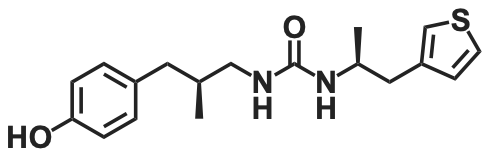
\includegraphics{PZM21.png}
	\caption{Structure of PZM21}
\end{marginfigure}

\begin{marginfigure}\label{fig:cxcrHM}
	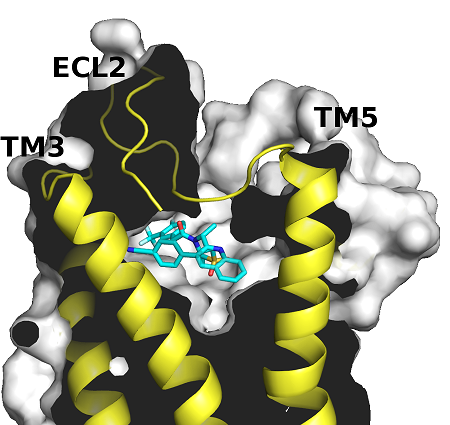
\includegraphics{cxcr3hpp_small.png}
	\caption{Homology model of CXCR3 with docked small molecule allosteric modulator.}
\end{marginfigure}
\newthought{Biased negative allosteric modulators of CXCR3.} Using homology modeling 
I constructed the structural model of CXCR3 based on X-ray structure of CXCR4 and
docked known allosteric modulators (ChEMBL) into the model. Thus we identified amino acid 
residues that regulate small molecule binding and downstream signaling. Attempts to engage 
a nucleophilic subpocket via reversible covalent interaction with strategically placed electrophilic boronic acid led
to discovery of the first biased negative allosteric modulator or CXCR3 (\textbf{14}, Fig. \ref{fig:cxcr3}).\cite{Bernat2014} 

Optimization of physico-chemical properties (cLogP and PSA) via introduction of flexible side
chain led to identificaiton of the negative allosteric modulator 
with the opposite signaling bias (\textbf{1b}, Fig. \ref{fig:cxcr3}). 
These biased modulators exhibited opposite probe dependence -- they preferentially
downregulated activation of CXCR3 by CXCL10 or CXCL11 chemokines.\cite{Bernat2015a} 
Affinities of these small-molecule allosteric modulators were similar (double-digit nM) as 
measured in radioligand RAMX3 displacement assay.\cite{Bernat2012}


Structural model of CXCR3 that I prepared was subsequently used \textit{as is} in virtual screening for identification
of completely novel chemotypes of specific and dual CXCR3 and CXCR4 allosteric modulators.\cite{Schmidt2015}

\newpage
\begin{fullwidth}
\phantomsection
\centering
\begin{figure*}
	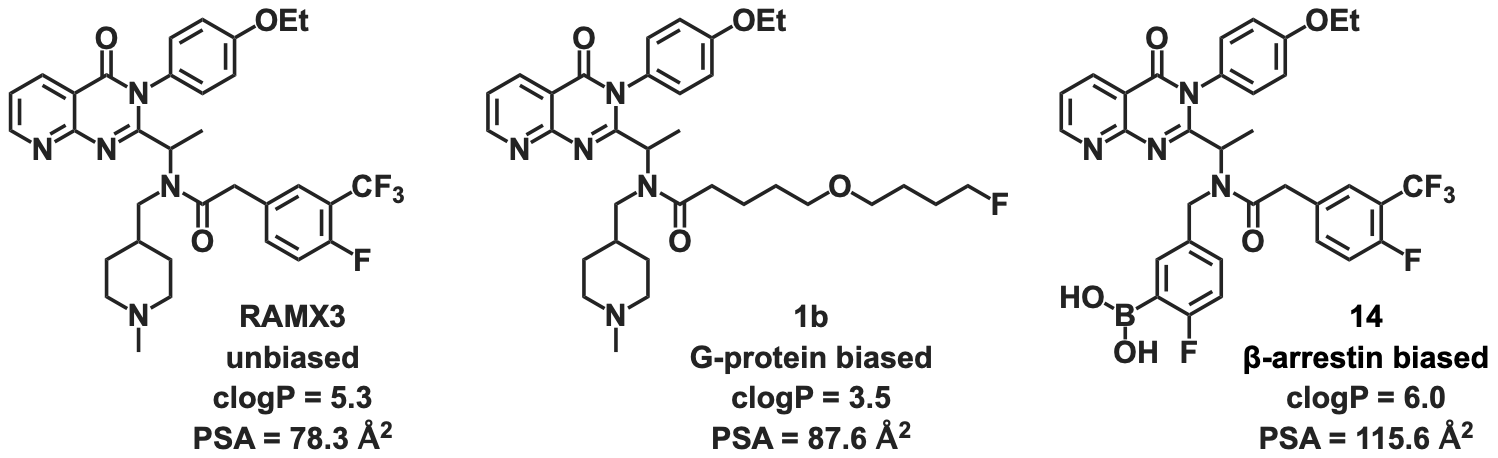
\includegraphics[height = 40mm]{cxcr3-allosteric-ligands.png}
	\captionof{figure}{Small molecule allosteric modulators of CXCR3}
	\label{fig:cxcr3}
\end{figure*}
\end{fullwidth}


\section{Chemical biology of non-coding RNA}
Non-coding RNA folds into 3D-structures that can be targeted by small molecules.\cite{Bernat2015b}
My research in chemical biology of RNA was about identification of new chemotypes targeting
pathogenic RNA structures and development of chemical tools for studying their role in
cellular markers of disease.
\begin{marginfigure}\label{fig:1a-TOq}
	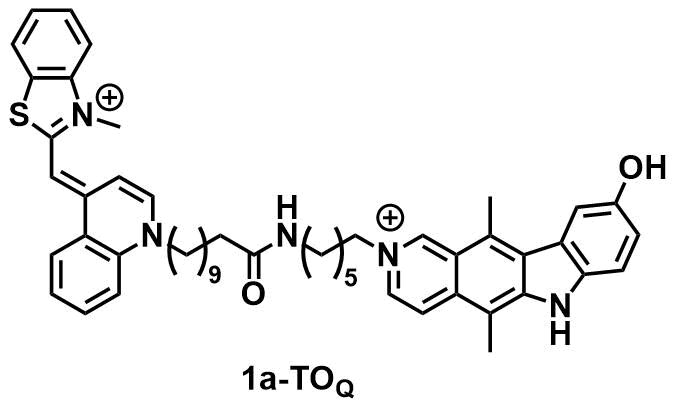
\includegraphics{1a-TOq.png}
	\caption{Fluorescent reporter for r(G4C2)\textsuperscript{exp} binding assay}
\end{marginfigure}
\newthought{Ellipticines as ligands for $r$(G4C2)\textsuperscript{ext}.} Building upon the previous work in the Disney lab, I developed fluorescent reporter 1a-TO\textsubscript{Q} which served as a tool for quick SAR interrogation \textit{in vitro} and led to discovery of better RNA binders from the same chemotype\cite{Wang2019}. Key insight was that permanent positive charge was not required for potent binding to RNA and activity in cellular assays. This dramatically improved blood-brain barrier penetration in mice.

\newthought{Chemical biology of $r$(CUG)\textsuperscript{exp} and $r$(CCUG)\textsuperscript{exp}.} To study the role of pathogenic non-coding RNAs in myotonic dystrophy I developed series of conjugates that disrupted interaction of r(CUG)\textsuperscript{exp} with proteins (GC-2H-CG, Fig. \ref{fig:kanamycin-dimers}\textcolor{DarkRed}{A}) or targeted the pathogenic r(CCUG)\textsuperscript{exp} for degradation by latent cellular nuclease RNAse L (Fig. \ref{fig:kanamycin-dimers}\textcolor{DarkRed}{B}). Further research in Disney lab built upon this work to develop microRNA degrading tool compounds.



\section{NIR fluorescent glucose sensors}

\begin{marginfigure}\label{fig:profusa}
	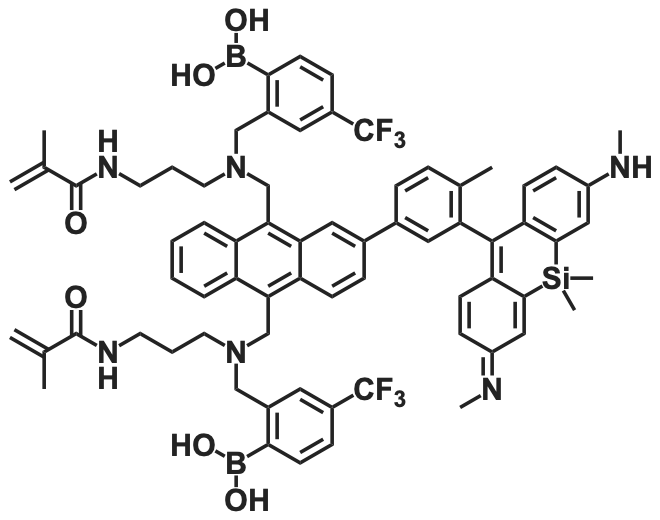
\includegraphics{v1dye.png}
	\caption{Example of glucose-sensing polymerizable NIR dye.}
\end{marginfigure}

At Profusa, I developed near-infrared (NIR) fluorescent sensors for continuous sensing of glucose \textit{in vivo}. The design of glucose sensors was based on known bis-boronic anthracene module that was incorporated into biocompatible hydrogel matrix. From a library of 120 dyes that I prepared\cite{Gamsey2018}, I could explore structure-activity relationships. Based on that I was able to rationally improve the performance of the company's prototype dye up to 5-fold. Finally, I scaled the synthesis of the lead dye to produce 1.8 g of material for clinical trials.

\begin{figure*}
	\phantomsection
	A)
	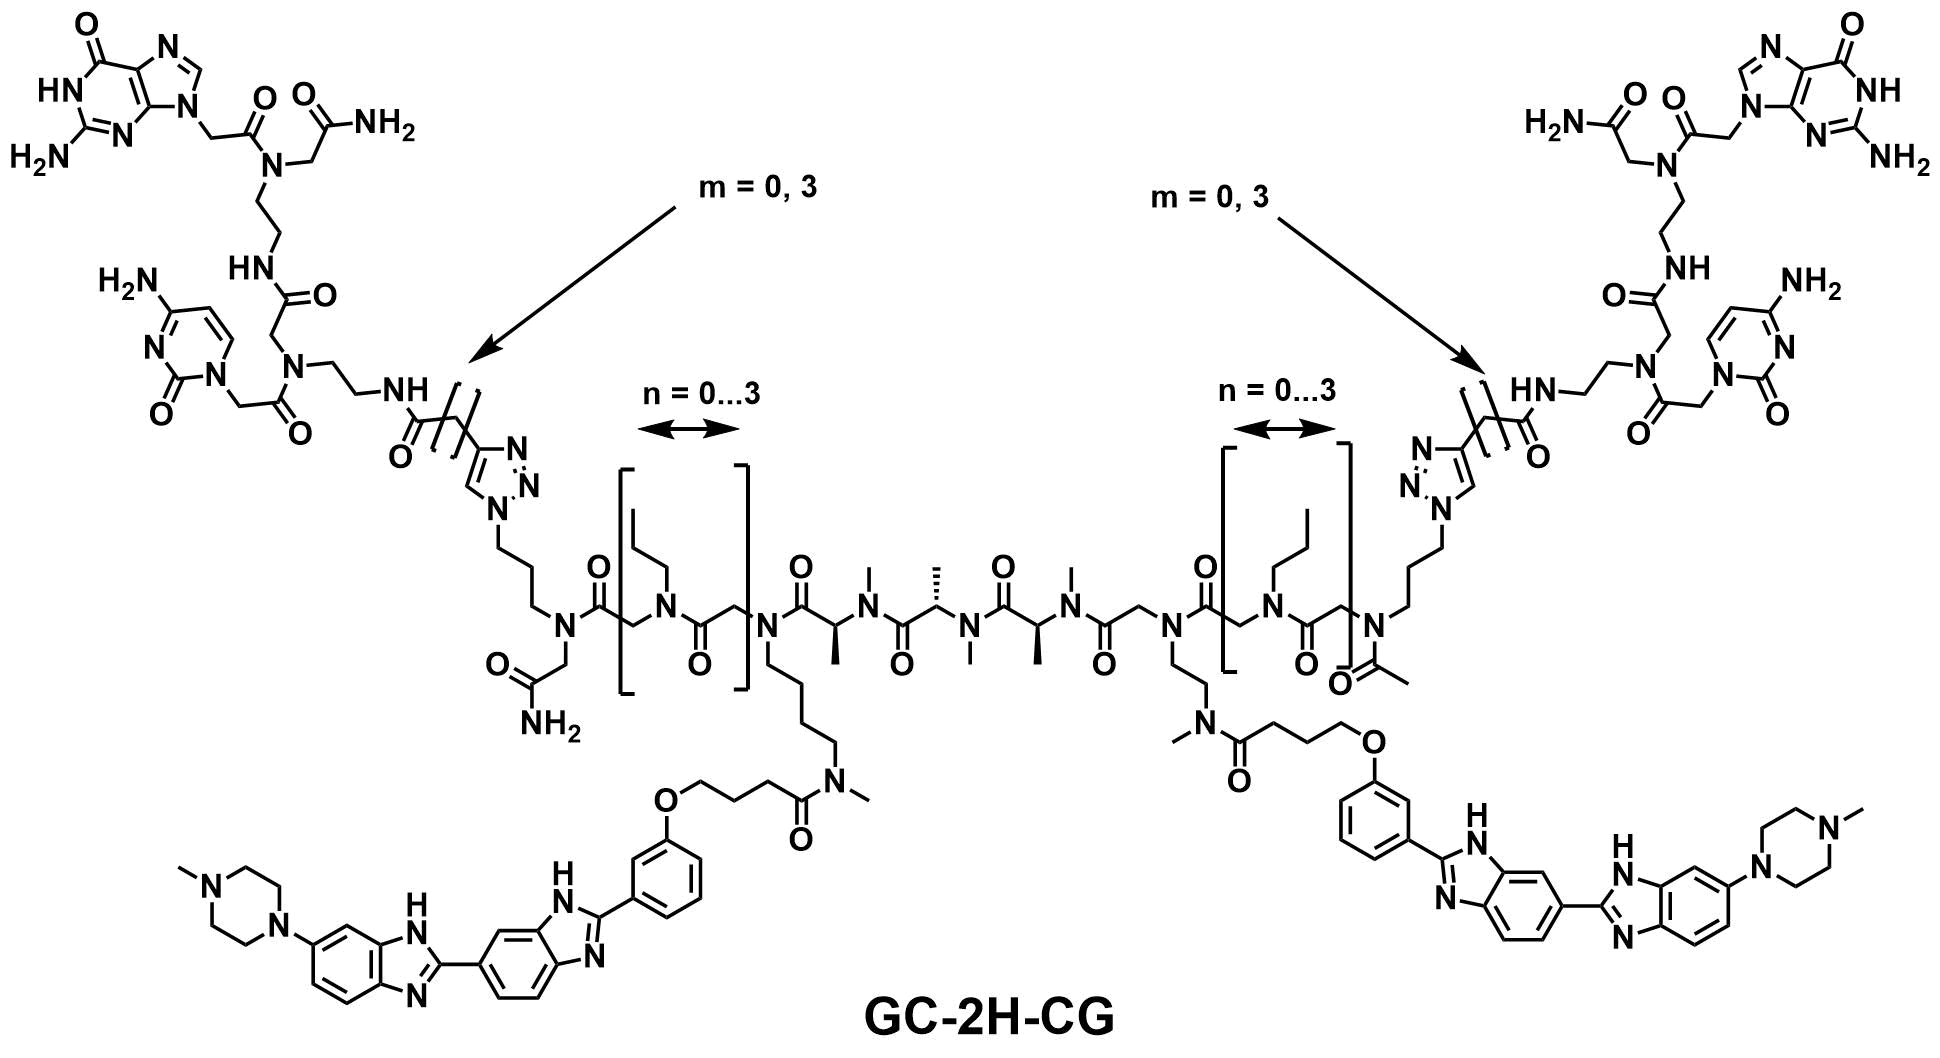
\includegraphics[width=80mm]{GC-2H-CG.png}
	B)
	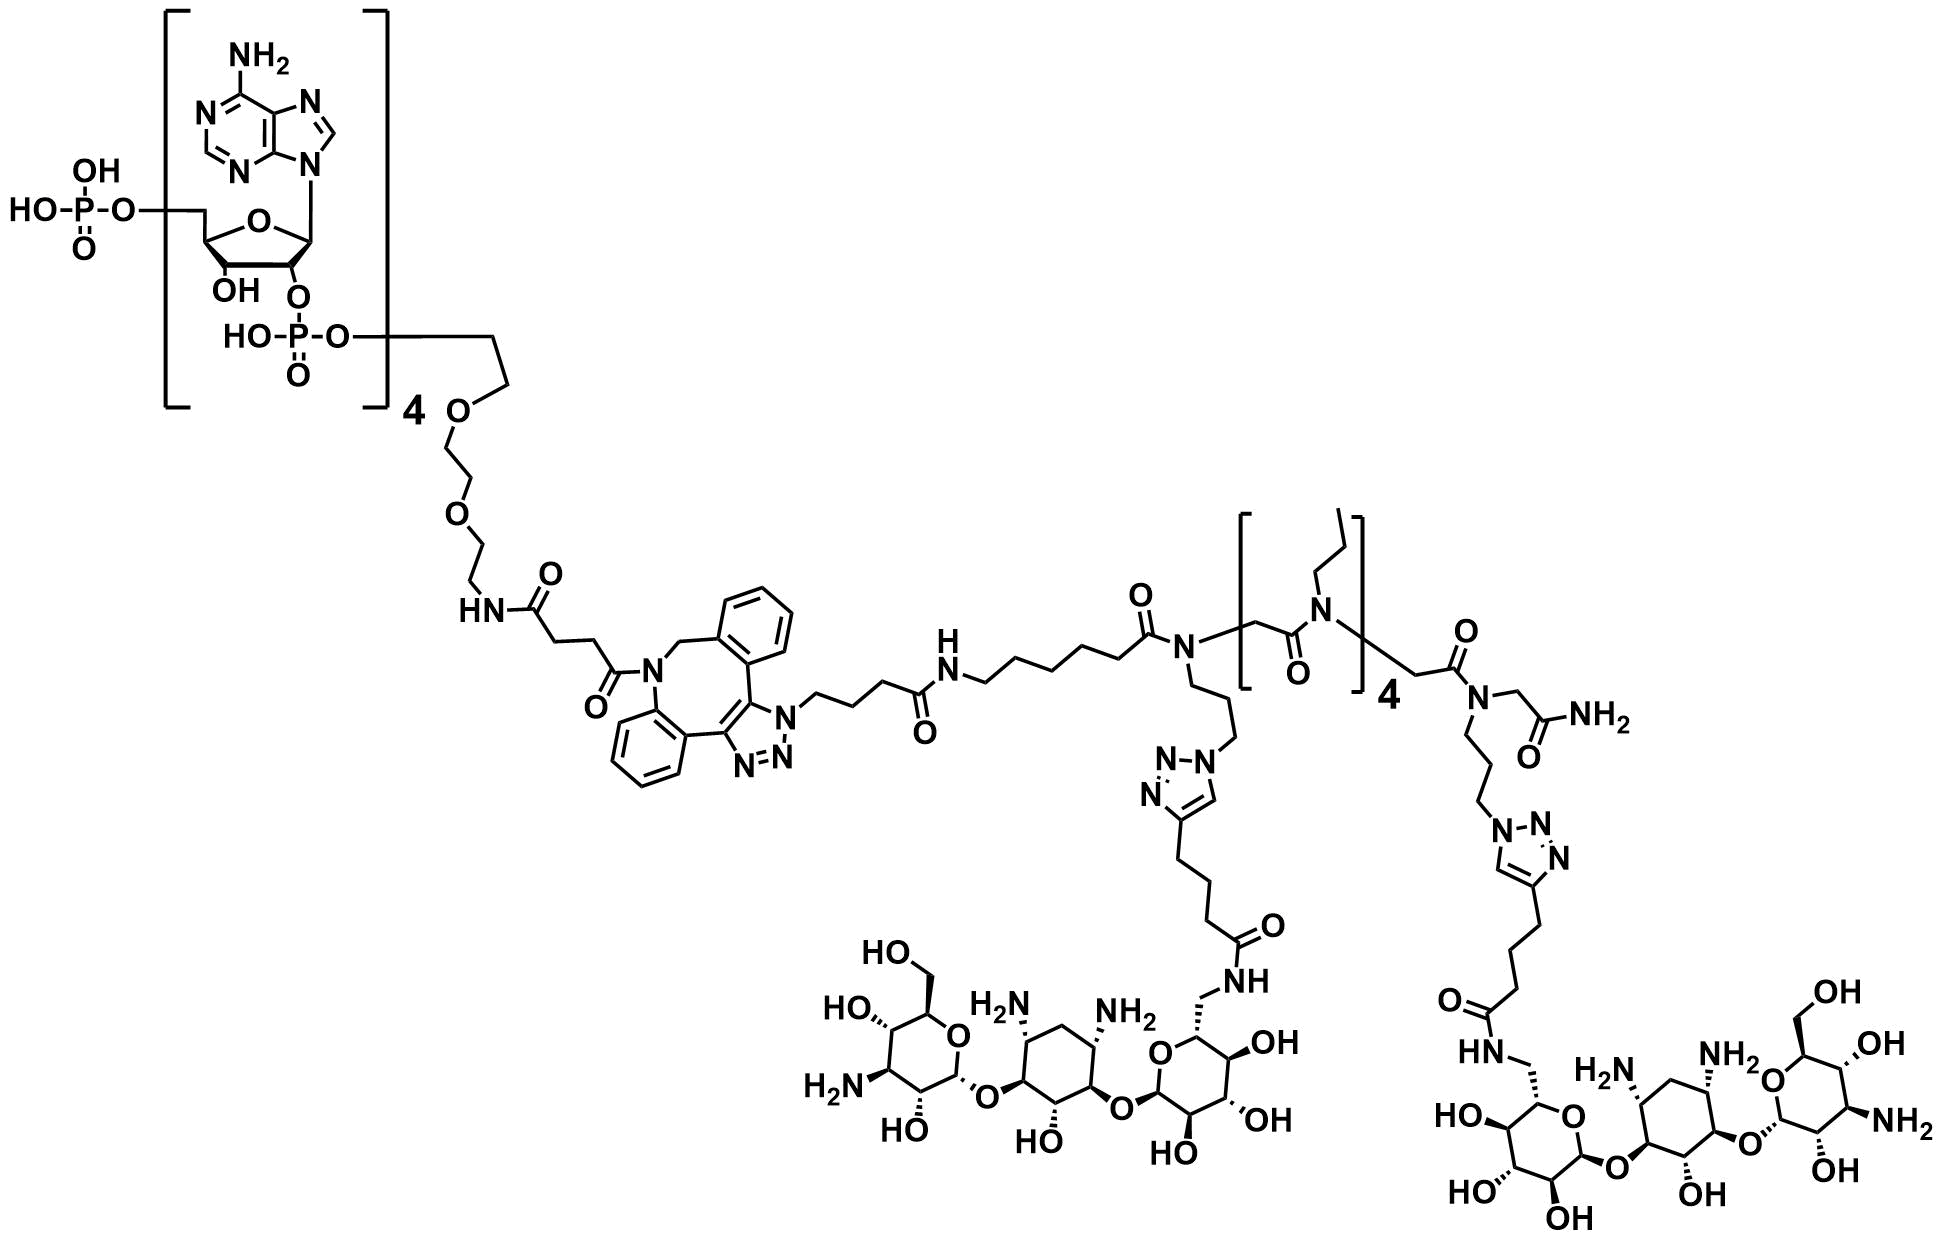
\includegraphics[width=80mm]{2Kan-p2-5A4.png}
	\caption{A) Structure of peptoid-PNA-Hoechst conjugate for disruption of r(CUG)\textsuperscript{exp} - MBNL1 interaction; B) Structure of peptoid-[2-5]A\textsubscript{4}-Kanamycin conjugate for targeting r(CCUG)\textsuperscript{exp} for degradation by RNAse L}
	\label{fig:kanamycin-dimers}
\end{figure*}


\bibliography{mypubs}
\bibliographystyle{plainnat}



\end{document}
